\documentclass{jib}
\newlength{\platz}
\setlength{\platz}{15pt}
\RequirePackage{listings}
\lstset{%
  basicstyle=\ttfamily,
  fontadjust,
  flexiblecolumns=true,
  frame=L,
  xleftmargin=15pt,
  framesep=5pt,
  emphstyle=\rmfamily\itshape}

\usepackage{pdfpages}

%%%%%%%%%%%%%%%%%%%%%%%%%%%%%%%%%%%%%%%%%%%%%%%%%%%%%%%%%%
% JIB Header/Footer
%%%%%%%%%%%%%%%%%%%%%%%%%%%%%%%%%%%%%%%%%%%%%%%%%%%%%%%%%%
\jibvolume{XX} % insert volume
\jibissue{X}   % insert issue
\jibpages{XXX} % insert article ID
\jibyear{XXXX} % insert year
\makeHeaderFooter{} % leave as is
%%%%%%%%%%%%%%%%%%%%%%%%%%%%%%%%%%%%%%%%%%%%%%%%%%%%%%%%%%

\begin{document}

%%%%%%%%%%%%%%%%%%%%%%%%%%%%%%%%%%%%%%%%%%%%%%%%%%%%%%%%%%
%
% Title Page
%
%%%%%%%%%%%%%%%%%%%%%%%%%%%%%%%%%%%%%%%%%%%%%%%%%%%%%%%%%%

\begin{jibtitlepage}

\jibtitle{The Simulation Experiment Description Markup Language (SED-ML):\\
Language Specification for Level~1 Version~4}


% Please make sure to use unique footnote characters for each author
\jibauthor{%
  Matthias K{\"o}nig\iref{humboldt},
  Frank T. Bergmann\iref{heidelberg},
  Lucian P. Smith\iref{uw},
  Alan Garny\iref{auckland},
  David Nickerson\iref{auckland},
  Dagmar Waltemath\iref{greifswald},
  Thomas Helikar\iref{nebraska},
  Jonathan Karr\iref{sinai} and
  Herbert Sauro\iref{uw}
}

%\addjibinstitution{imbio}{IMBio, Ralf Hofest\"adt, Bielefeld University, Faculty of Technology, Bioinformatics Department, D-33501 Bielefeld, Germany, \url{http://www.imbio.de}}
\addjibinstitution{humboldt}{Humboldt University, Germany}
\addjibinstitution{heidelberg}{BioQUANT/COS, Heidelberg University, Germany}
\addjibinstitution{uw}{University of Washington, USA}
\addjibinstitution{auckland}{Auckland Bioengineering Institute, The University of Auckland, New Zealand}
\addjibinstitution{greifswald}{University of Greifswald, Germany}
\addjibinstitution{nebraska}{University of Nebraska, USA}
\addjibinstitution{sinai}{Icahn School of Medicine at Mount Sinai, USA}

\end{jibtitlepage}


% adjusts the width of the abstract, please do not change!
%\begin{adjustwidth}{}{1cm} %LS NOTE:  'adjustwidth' not recognized in my setup.

\renewcommand{\baselinestretch}{1.0}
\abstract{
The use of computational simulation experiments to inform modern biological research creates new challenges to annotate, archive, share and reproduce such experiments.  Such simulations increasingly require extensive collaboration among modelers, experimentalists, and engineers. The Minimum Information About a Simulation Experiment (MIASE) guidelines outline the information needed to share simulation experiments. SED-ML is a computer-readable format for the information outlined by MIASE, created as a community project and supported by many investigators and software tools.

The first versions of SED-ML focused on deterministic and stochastic simulations of models.  Level~1 Version~4 of SED-ML substantially expands these capabilities to cover additional types of models, model languages, parameter estimations, simulations and analyses of models, and analyses and visualizations of simulation results. To facilitate consistent practices across the community, Level~1 Version~4 also more clearly describes the use of SED-ML constructs, and includes numerous concrete validation rules.

SED-ML is supported by a growing ecosystem of investigators, model languages, and software tools, including eight languages for constraint-based, kinetic, qualitative, rule-based, and spatial models, over 20 simulation tools, visual editors, model repositories, and validators. Additional information about SED-ML is available at \url{https://sed-ml.org/}.}

%\end{adjustwidth} % please do not change %LS NOTE:  'adjustwidth' not recognized in my setup.


% Include your PDF document
\clearpage
\setlength{\voffset}{0cm}
\setlength{\hoffset}{0cm}
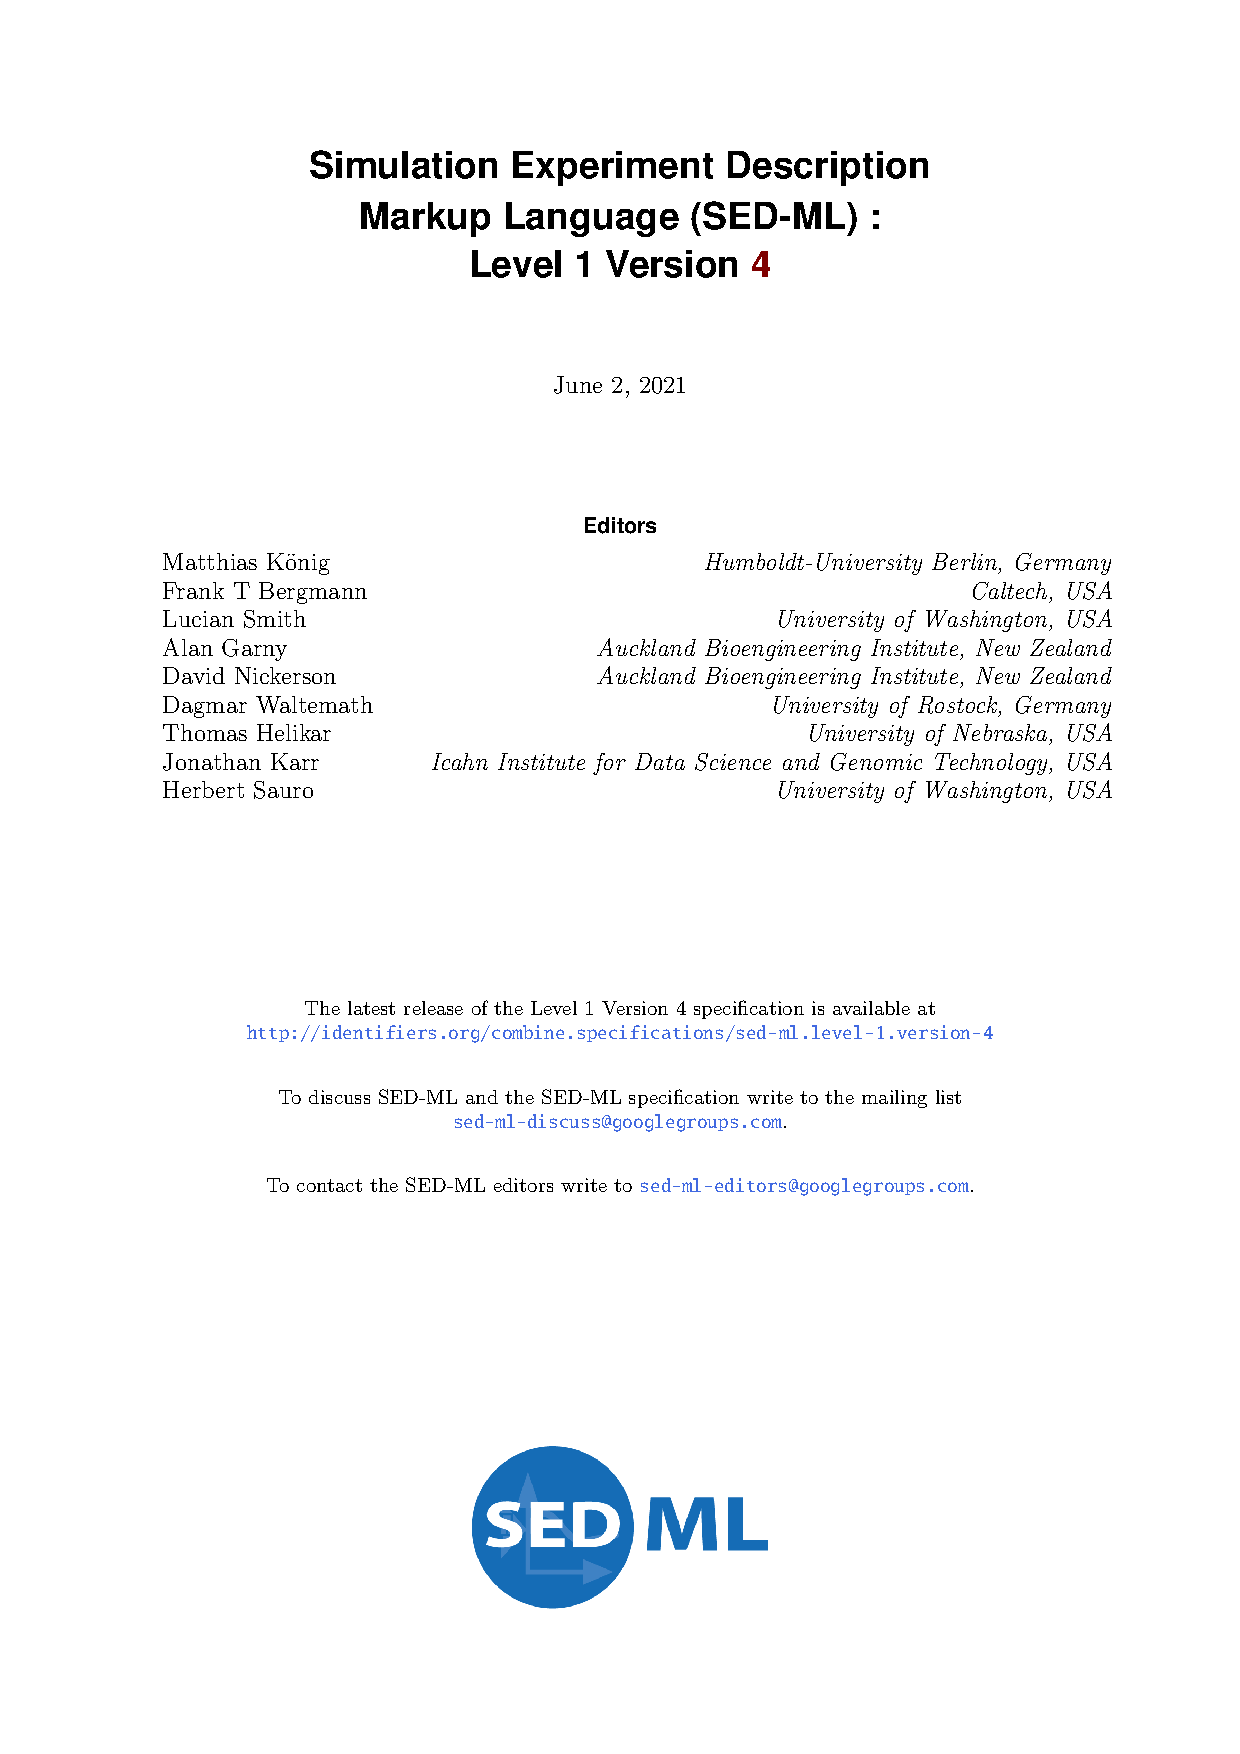
\includepdf[pages=-]{sed-ml-L1V4.pdf}

\end{document}
